\documentclass{article}
\usepackage{fontspec}
\usepackage{polyglossia}
\setdefaultlanguage{french}
\usepackage[a4paper,margin=1cm]{geometry}

\usepackage{amsmath}
\usepackage{amssymb}
\usepackage{array}
\usepackage{auto-pst-pdf}
\usepackage{booktabs}
\usepackage{cite}
\usepackage{graphicx}
\usepackage{lmodern}
\usepackage{marvosym}
\usepackage{mathrsfs}
\usepackage{minted}
\usepackage{multicol}
\usepackage{multirow}
\usepackage{paralist}
\usepackage{schemabloc}
\usepackage{siunitx}
\usepackage{soul}
\usepackage{tikz}
\usepackage[european,cuteinductors,siunitx]{circuitikz}
\usepackage{url,hyperref}
\usepackage{verbatim}
\usepackage{xunicode,xltxtra}

\title{
\includegraphics{../../../images/inp-enseeiht} \\ ~ \\ ~ \\ ~ \\ ~ \\ TP Convertisseur DC-DC}
\author{François Pierron \& Guilhem Saurel}
\date{\oldstylenums{\today}}

\begin{document}

\begin{titlepage}
    \setcounter{page}{0}
    \maketitle
    \vfill
    \tableofcontents
    \thispagestyle{empty}
\end{titlepage}


\section{Open Loop Study}

\paragraph{Observe the currents I(L), I(D1) et I(S1). Explain the behavior of currents according to the gate signal. In what mode are you ??}

~

~

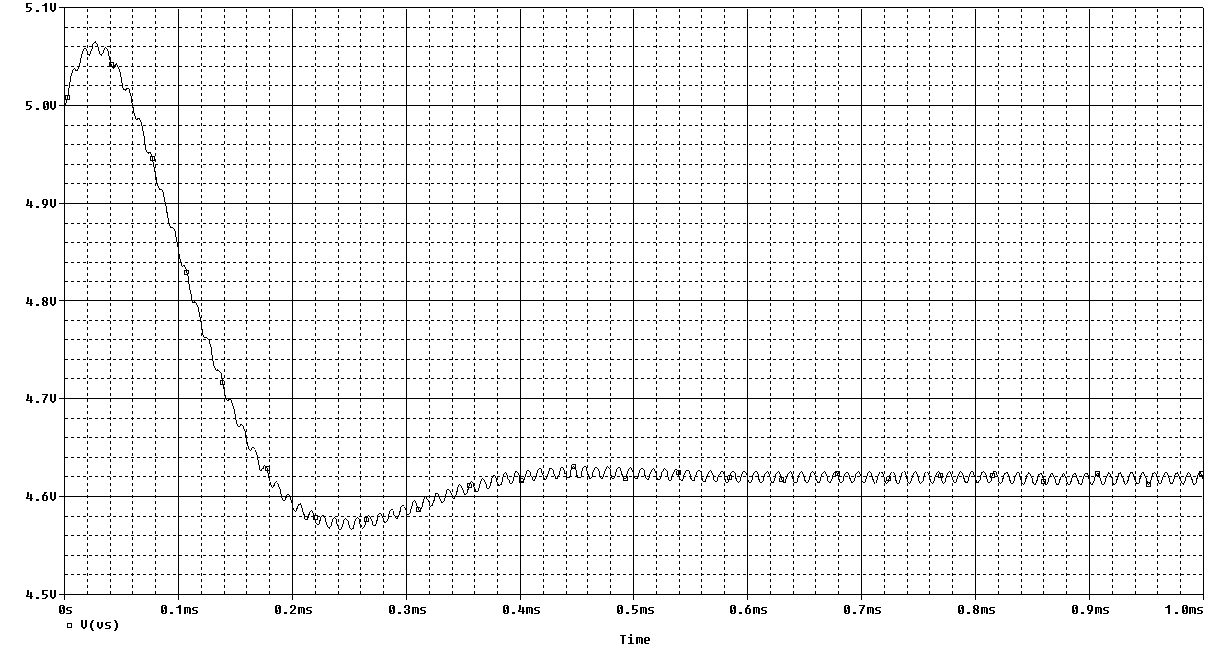
\includegraphics[width=\linewidth]{vs.png}

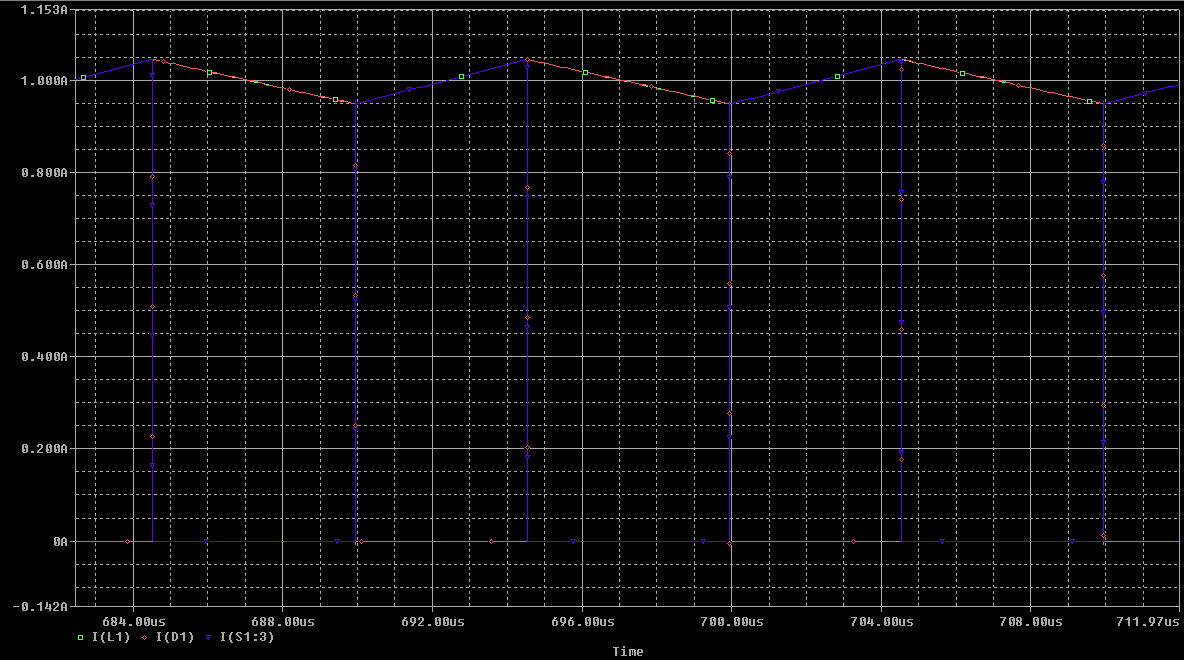
\includegraphics[width=\linewidth]{courants.png}

\newpage

\paragraph{Observe the control signals: Vrampe, Verreur, Vgrille and the resulting switched voltage Vk.}

~

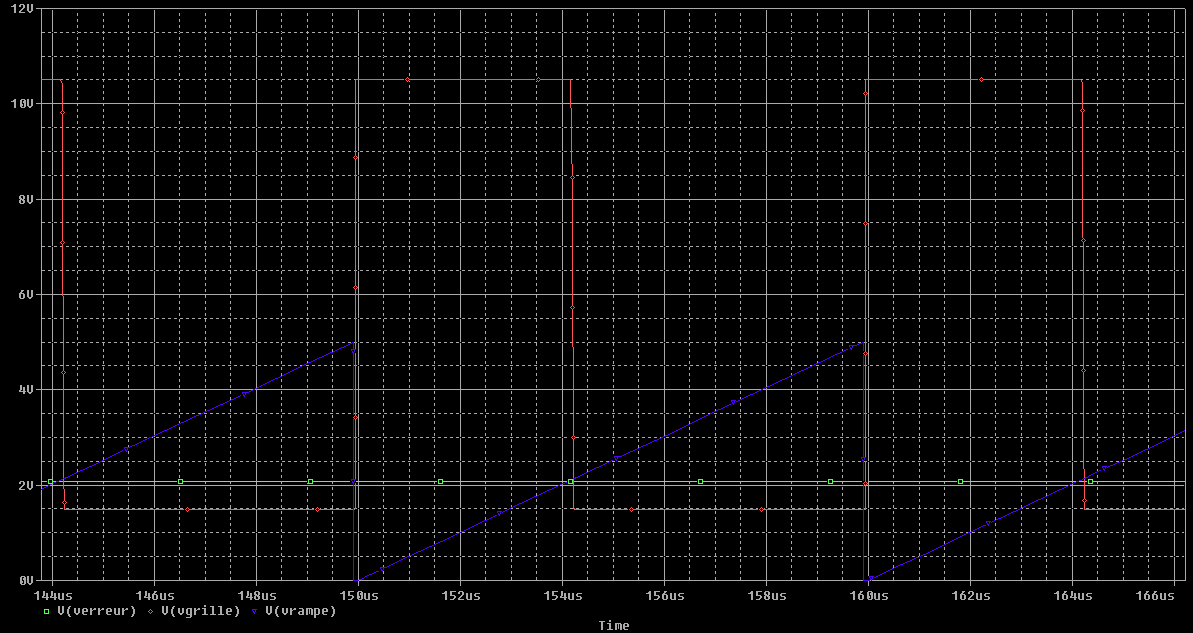
\includegraphics[width=\linewidth]{commandes.png}

\subparagraph{What is the value of the duty-cycle ?}

~

En théorie, cette valeur vaut $\cfrac{V_S}{V_{bat}} = \cfrac{5}{12} = 0.416$.

En pratique, on a $0.427$.

\subparagraph{Why do not you get exactly 5V for the voltage Vs by imposing D=5V/12V?}

~

La diode en inverse impose un abaissement de l’état bas du rapport cyclique de $V_D$. $V_S$ a donc une tension approximativement de $5-\cfrac{V_D}{2}$.


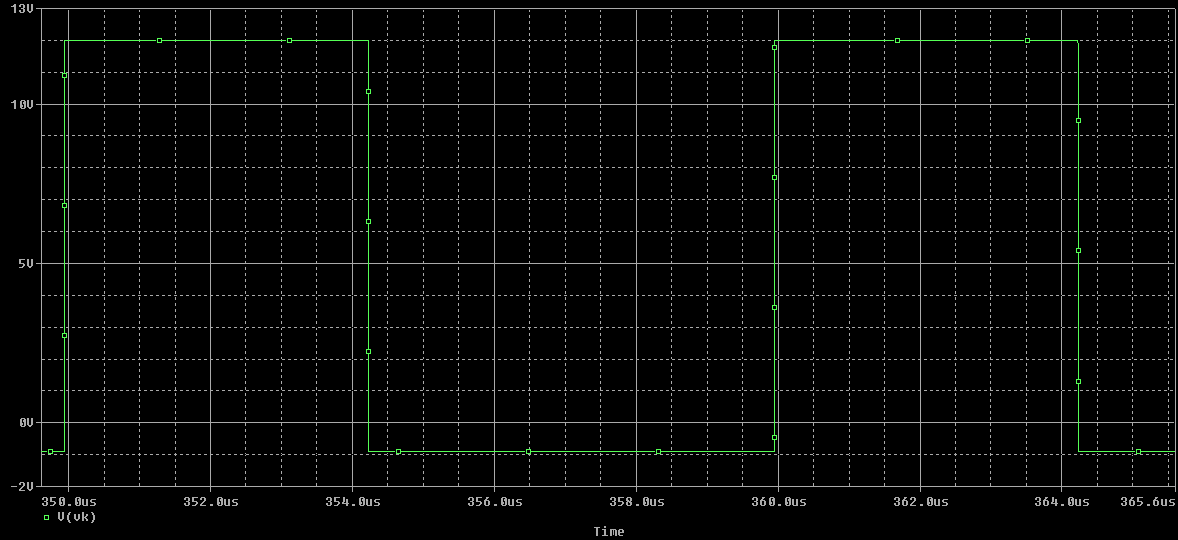
\includegraphics[width=\linewidth]{vk.png}

\subparagraph{Provide the expression of Vs=f(D,Vbat,Vd) avec Vd: knee voltage of the diode.}

~

$V_S = D V_{bat} - (1 - D)V_d$

\subparagraph{Deduce the voltage value to be imposed on Verreur to get Vs=5V.}

~

$V_{erreur}=2.22$V

\subparagraph{Check with a simulation.}

~

Après simulation, il semble que 2.235 corresponde mieux.

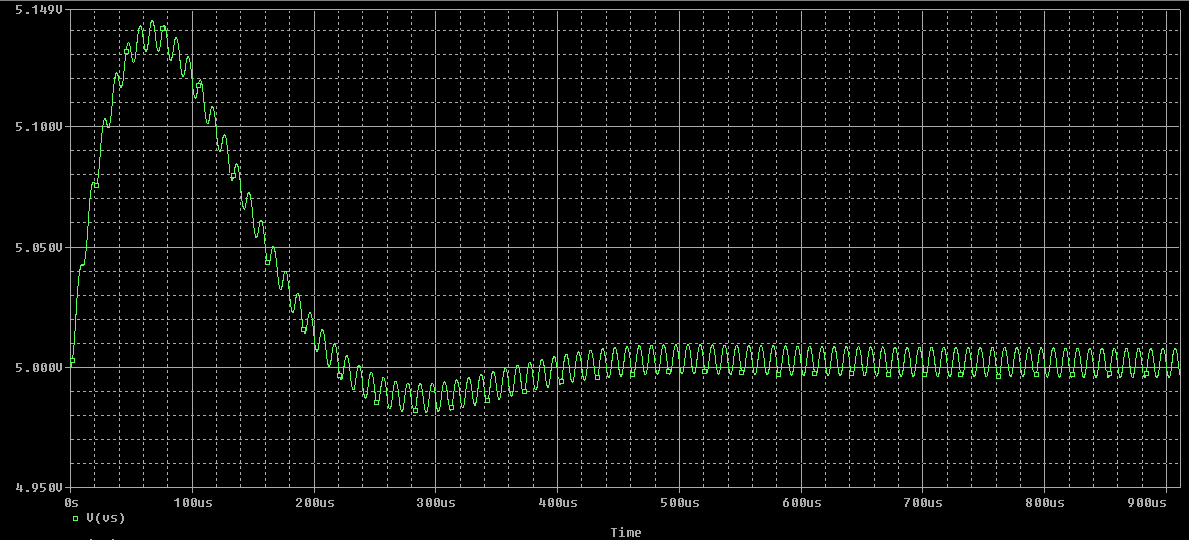
\includegraphics[width=\linewidth]{vs223.png}

\paragraph{Measure the value of the current ripple and the output voltage ripple and compare with the theorical values.}

~

$\Delta I_L = \cfrac{D(1-D)V_{bat}}{Lf_{dec}} = 0.0899$ A

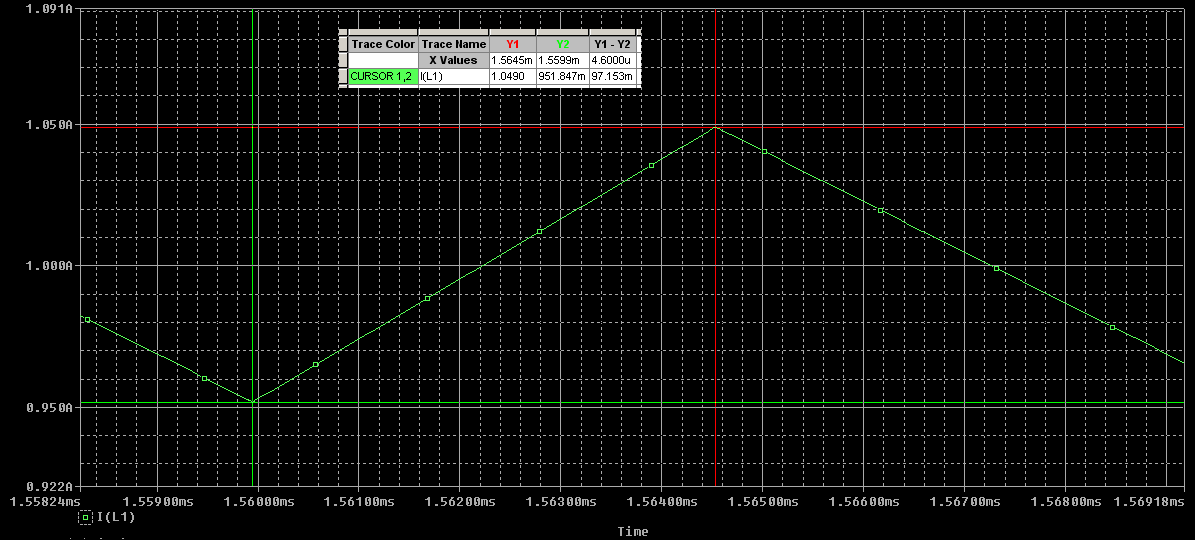
\includegraphics[width=\linewidth]{ripple_il.png}

En pratique, on est à 97mV.

$\Delta V_S = \cfrac{\Delta I_L}{8Cf_{dec}} = 0.0112$ V

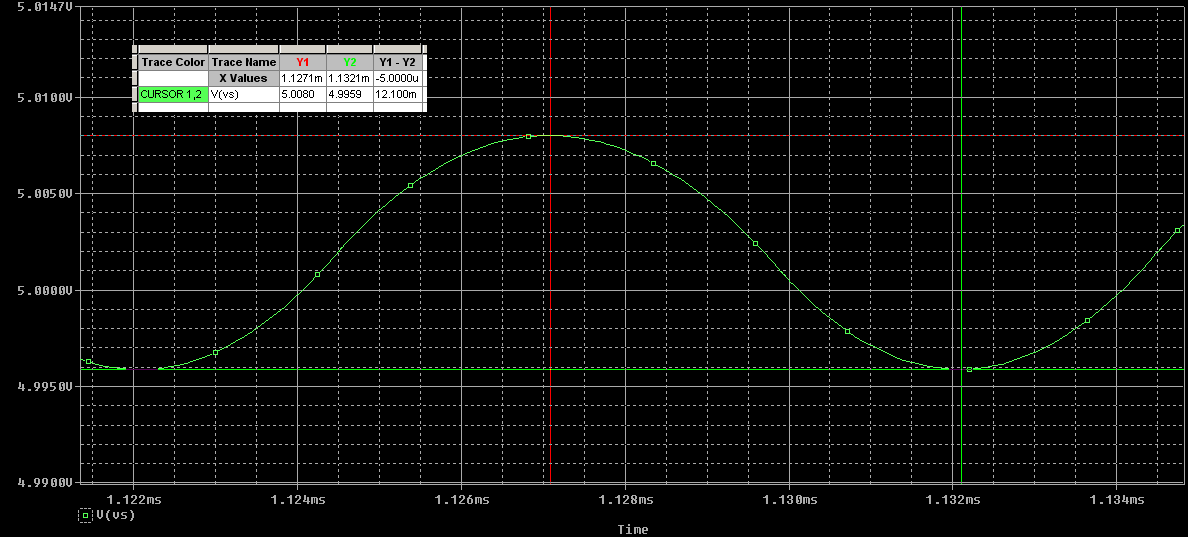
\includegraphics[width=\linewidth]{ripple_vs.png}

En pratique, on est à 12mV.

Donc dans les deux cas, la pratique est assez proche de la théorie.

\paragraph{By varying the load, check that the boundary separating modes is obtained for $R_{ch_{limite}} = \cfrac{2Lf}{1-D}$ with f: switching frequency (100kHz)}

~

La résistance limite entre les modes continu et discontinu est telle que le courant moyen de sortie est egal à la moitié du courant de ripple:
$R_{ch_{lim}} = \cfrac{V_S}{\cfrac{\Delta I_L}{2}} = 111\Omega$.

\subparagraph{Compare theory and simulation for both voltage: Vbat=12V and Vbat=20V}

~

On trouve que $V_D \simeq 0.9$V, donc, en théorie, on a $D = \cfrac{V_S-V_D}{V_{bat}-V_D}$.
Ceci conduit à des valeurs theoriques des résistances de $121 \Omega$ à 12V et de $91 \Omega$ à 20V ; et nous obtenons bien $117\Omega$ dans le premier cas, et $103\Omega$ dans le second.


\paragraph{In discontinuous mode, for Vbat=12V, Rcharge=300$\Omega$ and D=0.46, measure Vs (in steady-state) and check the expression
    $D=\cfrac{V_s}{V_{bat}}\cdot\sqrt{\cfrac{2Lf}{R_{charge}\left(1-\cfrac{V_s}{V_{bat}}\right)}}$.}

~

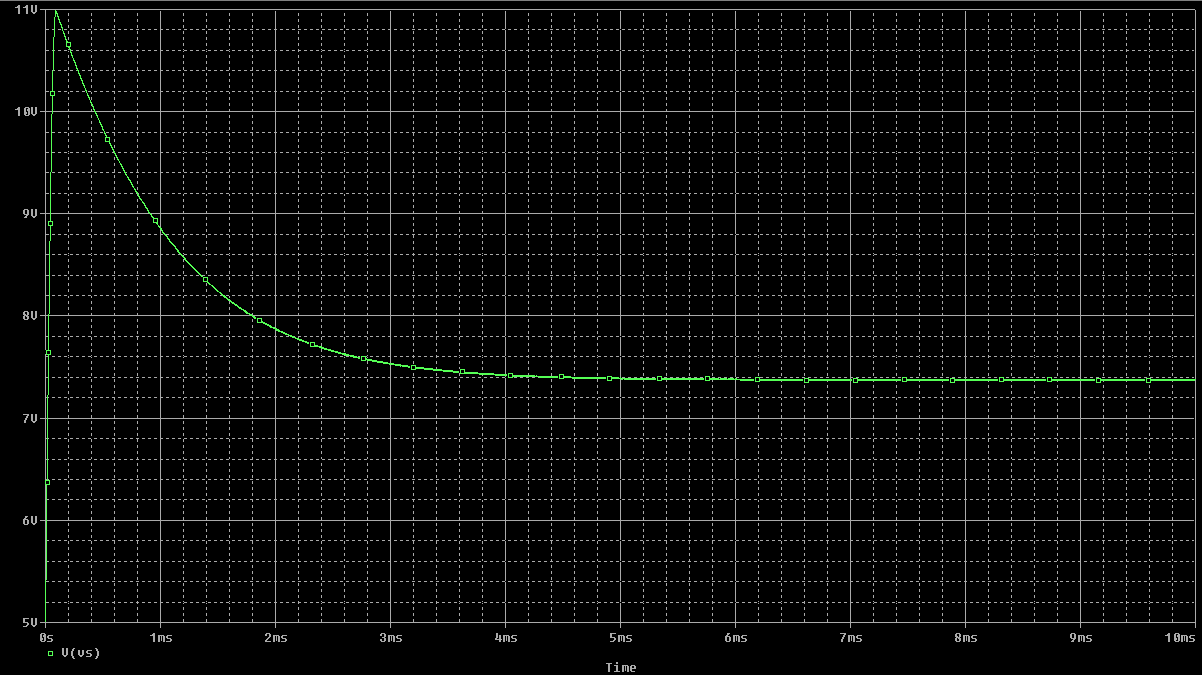
\includegraphics[width=\linewidth]{discontinuous.png}

$V_S=7.38$V, donc $D=0.46$


\paragraph{Observe (in simulation) the value of the overall efficiency of the circuit close to the nominal point (5V - 1A).}

~

La moyenne du courant consommé sur l’interrupteur est de 465mA
La moyenne du courant consommé par la résistance de charge est de 996mA pour une tension 4.98 V, ce qui fait à peu près 4.96W, d’où un rendement de 0.90.

\section{Boucle fermée: Étude de stabilité}

\paragraph{Calculez les valeurs des composants R1, C1, R2, C2 et C3}
On commence par déterminer $f_C = \cfrac{F_S}{10} = 5$kHz.
Ensuite, il faut obtenir $R_1C_1=\cfrac{1}{2\pi f_C} = 31.8\mu$s.
Pour cela, on peut fixer $R_1$ à 100 $\Omega$, et donc $C_1 = 318$nF.

~

Après, on cherche $R_2$, grâce au gain unitaire à $f_C$: $R_2=\cfrac{\left(2\pi f C\right)^2V_PLCR_1}{V_i} \simeq 1.8 $ k $\Omega$
(on prend $V_i$ à 6V parce qu’on se place dans le pire cas, c’est à dire celui où la marche de phase est la plus petite)

~

Enfin, on a $C_2$ grâce à la relation $C_2=\cfrac{1}{0.1R_2\sqrt{\cfrac{1}{LC}}} \simeq 820$ nF.

~

Pour finir, pour annuler l’effet ESR, on prend $C_3=\cfrac{ESR\cdot C}{R2}=55$pF.

~

~

On obtient donc le circuit suivant:

%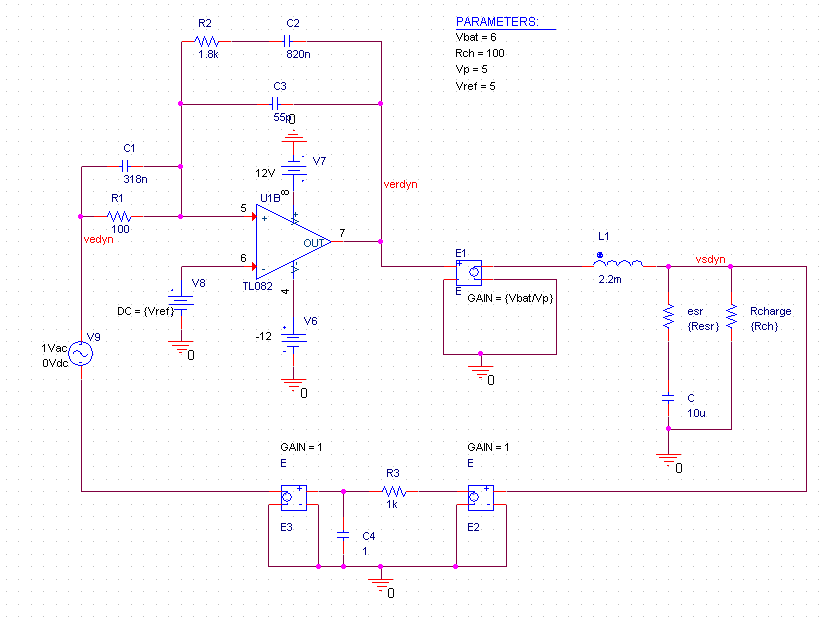
\includegraphics[width=\linewidth]{circuit_freq.png}

\paragraph{Faire un schéma équivalent pour obtenir le diagramme de Bode}

~

~

%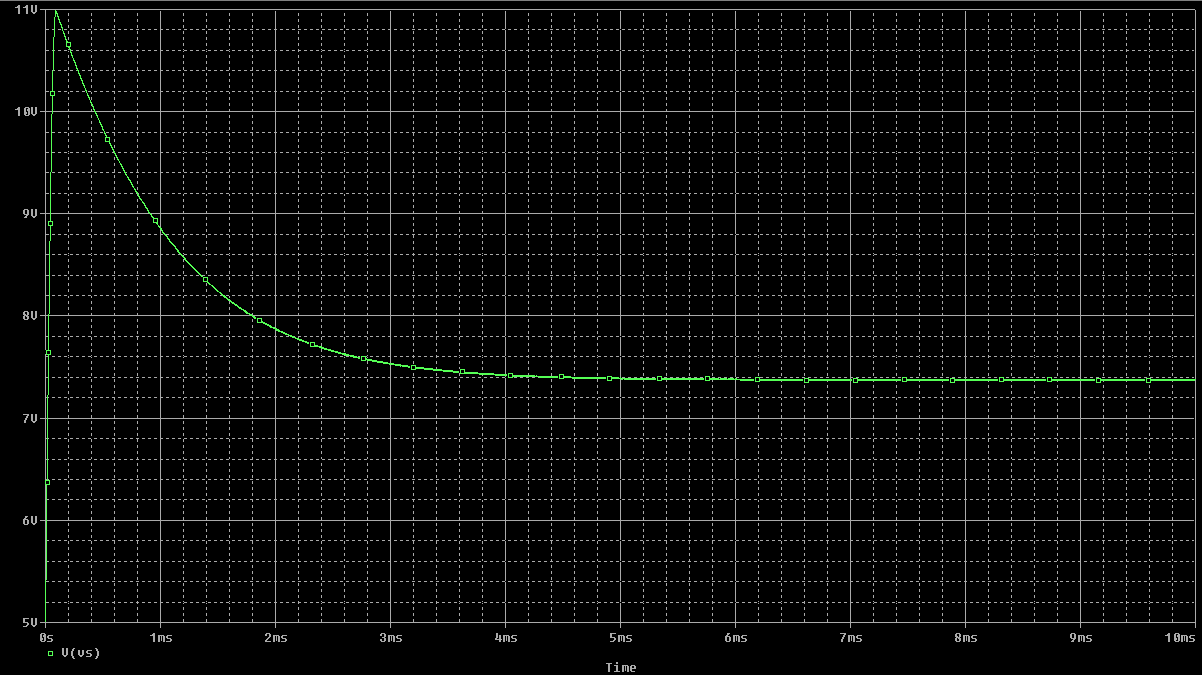
\includegraphics[width=\linewidth]{discontinuous.png}

~

\paragraph{Simulez (en fréquentiel et en temporel) et montrez que le système obtenu est stable dans les cas suivants: Vbat de 6V à 20V et Rcharge de 6 $\Omega$ à 100 $\Omega$.}

\paragraph{Donner deux tableaux donnant la marge de phase et l’atténuation à fs obtenus dans les 4 cas (Vbat, Rcharge).}

+================+=============+===============+
| Marge de phase | Rcharge = 6 | Rcharge = 100 |
+================+=============+===============+
| Vbat = 6V      |
+----------------+-------------+---------------+
| Vbat = 20V     |
+----------------+-------------+---------------+

+================+=============+===============+
| Atténuation    | Rcharge = 6 | Rcharge = 100 |
+================+=============+===============+
| Vbat = 6V      |
+----------------+-------------+---------------+
| Vbat = 20V     |
+----------------+-------------+---------------+



\end{document}
